\newpage
\section{Sistema de respuesta a preguntas (Q\&A)}

\subsection{Descripción del problema}

Los sistemas de respuesta a preguntas (o Q\&A por sus siglas en ingles) integran tareas de recuperación de la información (IR) y procesamiento del lenguaje natural (NLP) para poder responder de forma automática a preguntas de un usuario. La primera tarea busca encontrar información relevante, que pueda contener la respuesta para el usuario (i.e. un documento), por medio de una herramienta de búsqueda. Ya con esta información (también llamada \textit{contexto}) un sistema de \textit{based QA} realiza la tarea de comprensión de lectura, con la cual se busca extraer la respuesta exacta a la pregunta del usuario.
Esta segunda tarea tienen como único objetivo encontrar un pasaje (\textit{p}) que responda a la pregunta (\textit{q}) dentro del (o los) documentos relevantes recuperados para la pregunta. \\

A pesar de los recientes y acelerados desarrollos en el campo del procesamiento de lenguaje natural, los sistemas de respuesta a preguntas existen desde la década de los 60s. En esta época los sistemas se dedicaban a responder únicamente preguntas de un dominio muy especifico como baseball o análisis geológico. No obstante, con la gran cantidad de información disponible y el poder computacional de hoy en día, se puede fácilmente acceder a grandes colecciones de datos que permiten construir sistemas de respuesta a preguntas de dominio abierto. Asimismo, se tienen modelos de NLP profundos que permiten resolver de mejor forma la extracción de la respuesta dado el contexto.

\subsection{Revisión del estado del arte}

Para resolver el problema de recuperación de la información (IR) existen enfoques que datan desde la década de los 70s. Vale la pena aclarar que para esta tarea en especifico se requiere un \textit{set} ordenado de documentos (\textit{ranked}) y no solamente una colección de documentos relevantes y otros no. De esta manera se obtienen \textit{scores} de similaridad entre documento y \textit{query} para poder ordenar los resultados de la búsqueda. Con esto en mente, el enfoque más sencillo es el de utilizar la similaridad coseno de modelo de Bag-of-Words (BOW) que representa tanto al \textit{query} como al documento. Mejoras a esta metodología incluyen pesar los documentos por frecuencia (\textit{tf-idf term weighting}) y puntuación de documentos (\textit{document scoring}) \cite{}. Hoy en día existen sistemas de IR bien establecidos como \textit{Lucene} \cite{lucene} y arquitecturas basadas en \textit{deep learning} para la recuperación de la información \cite{DL_IR}. \\

Por otro lado, los sistemas de comprensión de lectura (o \textit{based QA}) del estado del arte utilizan como base modelos contextuales profundos pre-entrenados como ELMo y BERT \cite{BertQA}. Esto se debe al gran desempeño que han demostrado estos modelos en un amplio espectro de tareas de NLP. Ahora bien, con el objetivo de adaptar estos modelos contextuales a la tarea especifica, se utiliza el \textit{dataset} de pregunta a respuestas de la universidad de Standford SQuAD \cite{squad}. De esta manera, se realiza un \textit{fine-tuning} del modelo de BERT para así, a partir de su representación de la entrada (contexto y pregunta), el modelo recupere el pasaje con la respuesta \cite{BERT_on_SQUAD}.

\subsection{Metodología de solución}

La metodología general para la solución del problema de respuesta a preguntas se presenta en la figura \ref{fig:qa_diag}. Para esto se utilizó un subset de datos recopilados para Covid. Dada la naturaleza de la tarea en cuestión, los documentos recopilados de las redes sociales Twitter y Reddit fueron descartados, pues estas no proveen un contexto adecuado para la respuesta de preguntas y muchas veces dan información que es engañosa o falsa. Adicionalmente, se recopilo información de autoridades en la materia que brinden información adecuada y verídica para un tema tan sensible como lo es el Covid. En total se recuperaron entre 100 y 200 documentos de las páginas oficiales de la WHO y la CDC. \\


\begin{figure}[H]
    \centering
    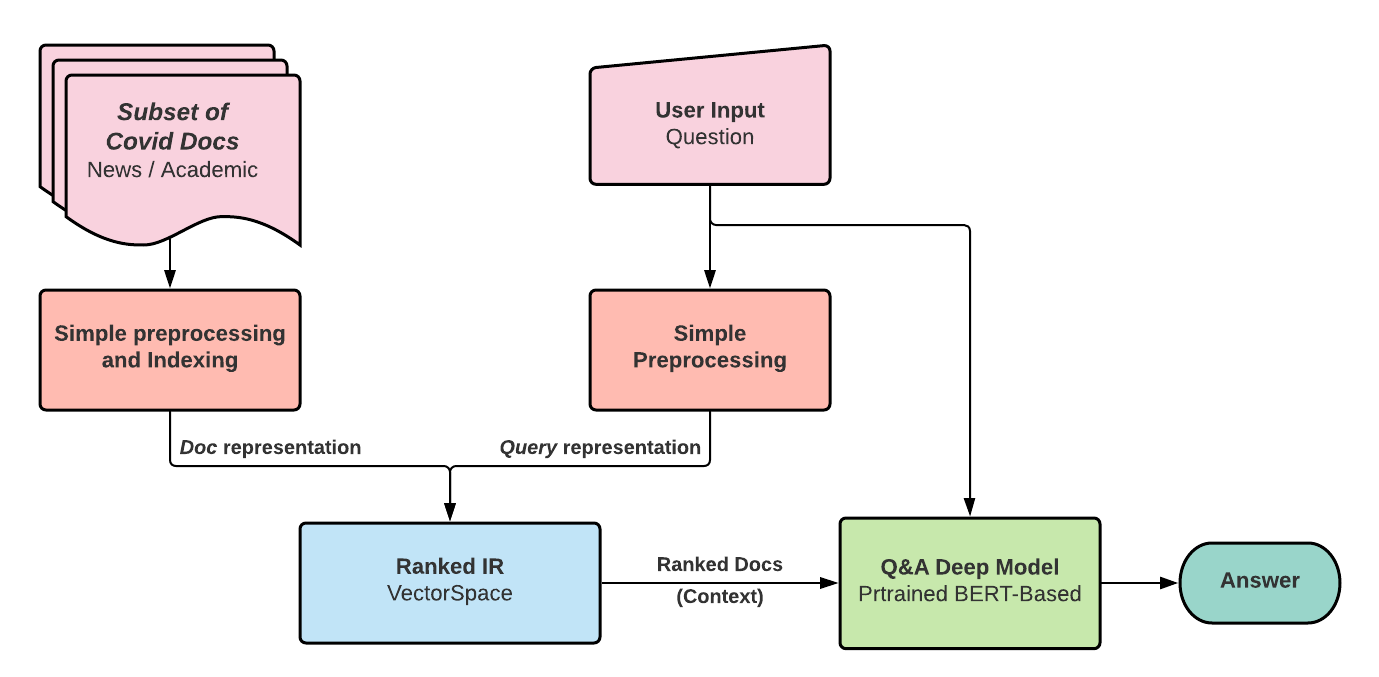
\includegraphics[width=0.85\textwidth]{doc_final/images/QA_System_diag.png}
    \caption{Flujo de información Sistema de respuesta a preguntas}
    \label{fig:qa_diag}
\end{figure}

A estos documentos se les realizó un pre-procesamiento estándar que incluye:
\begin{itemize}
    \item \textbf{lower case:} Las letras de todos los términos se transformaron a minúsculas.
    
    \item \textbf{tokenización:} Se tokenizaron las palabras con el tokenizador \texttt{RegexpTokenizer} de \texttt{nltk}, el cual elimina todo signo de puntuación.
        
    \item \textbf{simple lematization:} Se redujo cada uno de los términos a su raíz con el lematizador \texttt{WordNetLematizer} de \texttt{nltk}.
\end{itemize}

\subsubsection{Information Retrieval}

Una vez se tienen los documentos preprocesados, se procede a construir, entonces, el sistema de recuperación de la información (IR) con la librería de \texttt{Gensim}. Esta implementación realiza una vectorización de documentos de forma sencilla con un modelo de Tf-idf (\texttt{TfidfModel()}) con el corpus de documentos. Se crea una matriz de similaridad ((\texttt{MatrixSimilarity()}) con el modelo de Tf-idf del corpus de documentos. Con esta matriz y el modelo de Tfidf se transforman cada una de las \textit{queries} y se realiza la recuperación de la información a partir de su similaridad de coseno (\textit{cosine similarity score)}, ordenando los resultados de mayor a menor similaridad. De igual forma, se tienen en cuenta únicamente los documentos con un puntaje (\textit{score}) mayor a 0. \\

Ahora bien, en este punto vale la pena mencionar, que se hicieron pruebas de todo el sistema de respuesta a preguntas utilizando tanto los títulos como el cuerpo como "documento" en la tarea de recuperación de la información. En este caso, fue mejor utilizar únicamente los títulos de los documentos recuperados. Sin embargo, al final es el cuerpo de estos documentos el que se pasa como contexto al modelo contextual profundo pre-entrenado. \\

\subsubsection{Q\&A Deep Model}

Ya con el contexto recuperado, se utiliza un modelo contextual pre-entrenado para la tarea de respuesta a preguntas (\textit{question-answering}), con el fin de extraer la respuesta como un pasaje del contexto. Para esto se consideraron los siguientes modelos:

\begin{itemize}
    \item Inglés: RoBerta-base SQuAD2.0 for QA on COVID-19
    
    \item Español: BETO (Spanish BERT) + Spanish SQuAD2.0
    
    \item Francés: CamemBERT model fine-tuned on FQuAD
\end{itemize}

Note que el modelo utilizado para inglés no solo se entrenó (\textit{fine-tuned}) con el \textit{dataset} para pregunta a respuestas SQuAD2.0 sino que también fue entrenado con un \textit{dataset} especifico para Q\&A en el dominio de COVID-19 \cite{moller-etal-2020-covid-qa}. Esto permite comparar la ventaja y el efecto que tiene realizar este entrenamiento extra (\textit{fine-tuning}) sobre el modelo contextual. \\ 

Finalmente, para entregar la respuesta al usuario, estos modelos entregan un nivel de confianza o puntaje (\textit{score)} que permite determinar que tan certera puede llegar a ser la respuesta. Con esto en mente, y a partir de un \textit{threshold}, se decide si la respuesta que se obtiene es lo suficientemente buena o si se requiere de revisar el siguiente documento recuperado en la lista ordenada que se tiene.

% --------------------------------------------------------------------
%                                RESULTS
% --------------------------------------------------------------------
\subsection{Resultados}

Finalmente, para poner a prueba el sistema de Q\&A propuesto e implementado se procede a realizar pruebas sobre estos modelos con un pequeño set de 10 preguntas construidas a mano a partir de las fuentes recuperadas (WHO y CDC). Los resultados de estas pruebas se pueden evidenciar en las figuras \ref{tab:results_es_qa} - \ref{tab:results_fr_qa}. \\

Adicionalmente, para estas pruebas se calcularon dos métricas típicas para evaluar el sistema de respuesta a preguntas: $Exact Match$ y $F1 Score$, la primera sencillamente evalúa si se obtuvo una respuesta exactamente igual a la esperada y la segunda es una medida que considera tanto \textit{precisión} y \textit{recall} a nivel de palabras con respecto a la respuesta original. Adicionalmente, también se tuvo en cuenta el número de documentos recuperados que fue necesario revisar antes de entregar una respuesta con un \textit{score} mayor al \textit{threshold} puesto (para todos los casos este se fijo en 0.1).

\begin{table}[H]
    \centering
    \caption{Resultados del sistema de Q\&A para español}
    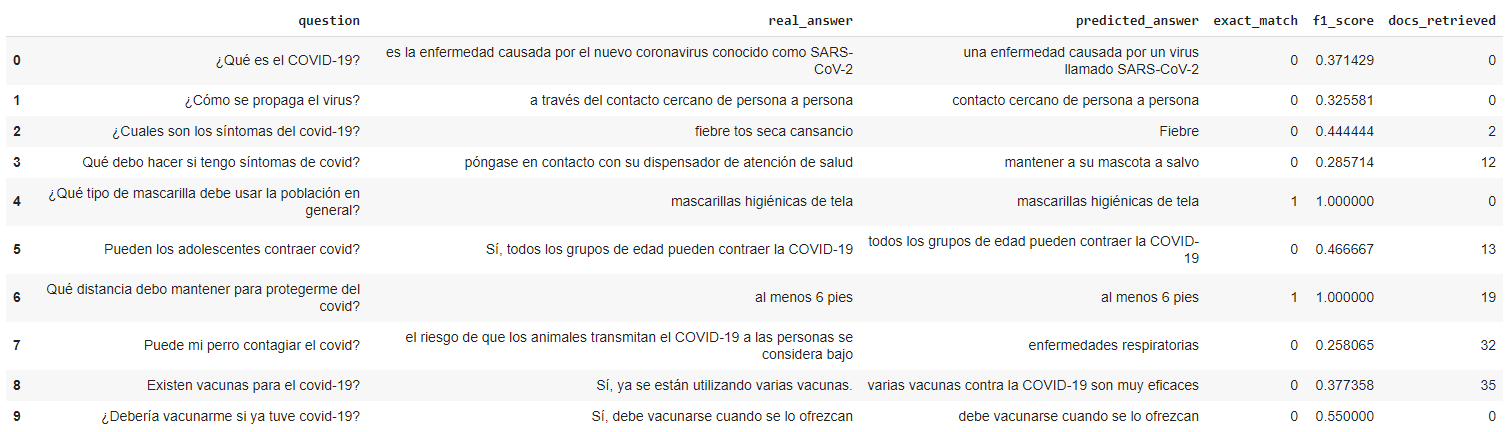
\includegraphics[width=\textwidth]{doc_final/images/qa_es_results.PNG}
    \label{tab:results_en_qa}
\end{table}

\begin{table}[H]
    \centering
    \caption{Resultados del sistema de Q\&A para inglés}
    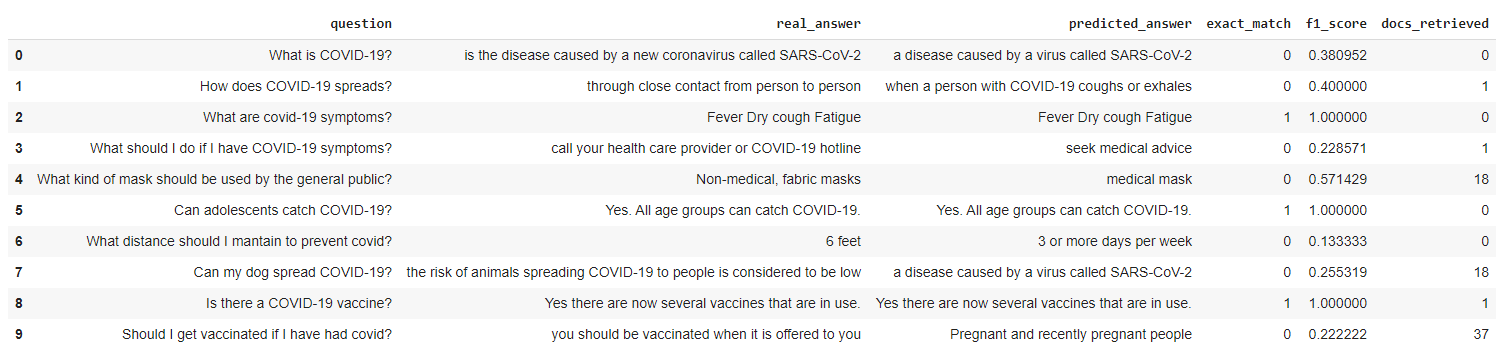
\includegraphics[width=\textwidth]{doc_final/images/qa_en_res.png}
    \label{tab:results_es_qa}
\end{table}

\begin{table}[H]
    \centering
    \caption{Resultados del sistema de Q\&A para francés}
    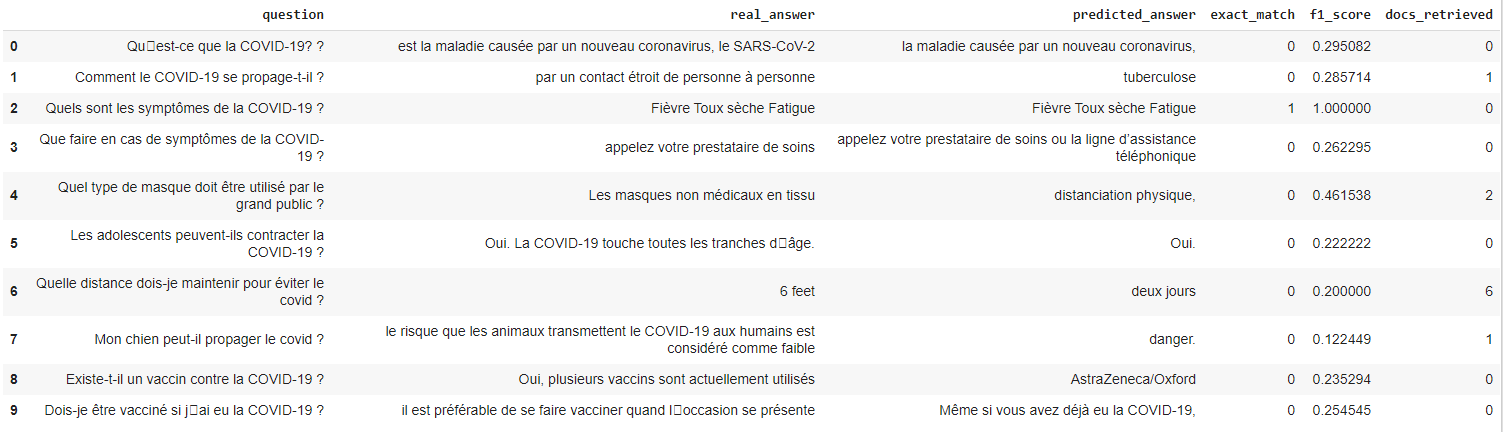
\includegraphics[width=\textwidth]{doc_final/images/qa_fr_results.PNG}
    \label{tab:results_fr_qa}
\end{table}

Finalmente, en la tabla \ref{tab:results_qa_summary} se presentan los resultados promediados para el pequeño \textit{dataset} de 10 preguntas.

\begin{table}[H]
\centering
\caption{Resultados promedio del sistema de Q\&A para los tres idiomas}
\begin{tabular}{|l|c|c|c|}
\hline
\multicolumn{1}{|c|}{\textbf{Lang}} & \textbf{Exact Match} & \textbf{F1 Score} & \textbf{Docs Retrieved} \\ \hline
\textbf{es}                         & 0.2                  & 0.5079            & 11.3                    \\ \hline
\textbf{en}                         & 0.3                  & 0.5192            & 7.6                     \\ \hline
\textbf{fr}                         & 0.1                  & 0.3339            & 1.0                     \\ \hline
\end{tabular}
\label{tab:results_qa_summary}
\end{table}

\subsection{Conclusiones}

A pesar de que las pruebas realizadas se realizaron sobre un dataset reducido, se puede apreciar tanto a un nivel cuantitativo como cualitativo un desempeño apropiado del sistema de respuesta a preguntas. Para las 10 preguntas propuestas se obtuvieron valores de las métricas bastante similares a lo que se esperan para este tipo de sistemas. Como referencia, los resultados del RoBerta-base SQuAD2.0 for QA on COVID-19 (utilizado para inglés) en el dataset de covid \cite{moller-etal-2020-covid-qa} evidenciaron resultados de entre 0.2 y 0.25 para $Exact Match$ y de 0.5 para $F1 Score$. Esto pues obtener una respuesta exactamente igual es realmente una tarea difícil. \\

Ahora bien, vale la pena aclarar que, para la implementación presentada, estas métricas se midieron incluyendo la etapa de recuperación de la información. Esto quiere decir que no se midieron a partir del contexto sino esperando que el sistema de IR recuperara el documento adecuado para responder la pregunta. Esto se evidencia en algunos resultados (especialmente en inglés) donde la respuesta podría considerarse como correcta a pesar de no serlo, como por ejemplo: en el caso de la pregunta \textit{"What should I do if have COVID-19 symptoms?"}, en donde la respuesta predicha fue \textit{"seek medical advice"}, que puede entenderse como correcta al lado de la respuesta real \textit{"call your health care provided"}. Esto puede deberse a que sencillamente se encontraron más datos y más información relevante tanto en la WHO como en la CDC para el idioma inglés, lo que sugiere una mayor cantidad de documentos (contextos) capaces de proveer la respuesta correcta. \\

Finalmente, al hacer el análisis a nivel de idiomas, adicional al efecto que puede tener el desbalance en la cantidad de datos utilizados, los resultados en cuanto a desempeño también son considerablemente diferentes. Por un lado el idioma inglés presentó los mejores resultados (y potencialmente un mejor desempeño por lo que se mencionó anteriormente), lo cual puede darse no solo a la cantidad de información que tiene disponible sino también dado que presentaba un modelo entrenado específicamente para esta tarea en este dominio. No obstante, los resultados del idioma español son muy similares, a pesar de no tener un \textit{fine-tuning} especifico para el dominio COVID, lo cual sugiere que el modelo de respuesta a preguntas puede funcionar bastante bien para un dominio especifico como el que se presentó en este caso. \\

Finalmente, los resultados del sistema en francés fueron los que presentaron el menor rendimiento a pesar de encontrar las respuesta en los primeros documentos encontrados (menor \textit{average retrieved docs}). Esto último sugiere que el parámetro de \textit{threshold} con el que se decide si una respuesta es lo suficientemente buena o no para buscar en otro documento es un parámetro que debe sintonizarse tanto para idioma como para modelo.

\newpage